\chapter{Features' importance}

After having determined the most performant algorithm, which is Random Forest, it is time to go further and analyse which features impact the results of classification the most. The focus will be especially on false predictions. In order to do that, six tools will be compared: LIME \cite{lime}, ELI5 \cite{mikhail_korobov_eli5_nodate}, YellowBrick \cite{bengfort_yellowbrick_2018}, Treeinterpreter \cite{ando_saabas_treeinterpreter_nodate}, dtreeviz \cite{terence_parr_dtreeviz_nodate} and export\_graphviz tool from scikit-learn, where the last three ones are designed for Decision Tree and Random Forest classifiers.

\section{Result's interpreters' comparison}
\subsection{LIME} %detaille plus
LIME (Local Interpretable Model-agnostic Explanations) is a tool that is used to explain the behaviour of machine learning classifiers. It supports, as for this day, only the explanation of individual predictions for any scikit-learn classifier or regressor. This explanation consist in a list of features ordered by their relative importance for a particular prediction. This list can be shown is a raw mode (as a python list) or in a visual form (pyplot figure, jupyter notebook or html file).

In order to class the features according to their importance, LIME approximates the model by an interpretable one, created based on perturbing the features of the examined instance. More the perturbed instances are similar to the examined instance, higher is the weight of the perturbed feature.

\subsection{ELI5}
ELI5 (Explain like I am a 5-year old) is a tool, in form of a Python package, used to debug machine learning classifiers and explain their predictions. It supports multiple machine learning frameworks, including scikit-learn. It can be used to explain how the model works both locally for one prediction and globally for the whole model. The output can take several forms just like in LIME case.

For white-box models, ELI5 works as an extension of scikit-learn and it's capable to extract the weights of model's features for different classes. In addition to that it can show the weights that contributed in a particular prediction. On the other hand, for black-box models, this tool integrates a modified version of LIME, supporting more machine learning frameworks, and a permutation importance method, which checks how the model's accuracy decreases when removing one of the features and on this basis determines the importance of the features.

\subsection{YellowBrick}
YellowBrick is another Python package, which is an extension of scikit-learn framework. It is meant to give global interpretation of the analysed model on different levels. It is possible not only to visualize features importances calculated directly by scikit-learn, but also to give a classification report (accuracy, recall, precision, f-measure), plot a confusion matrix, a ROC curve and much more. In addition to all that, YellowBrick comes with a tool for determination of correlation between features in the dataset.

\subsection{Treeinterpreter}
Treeinterpreter is a simple Python package that works with scikit-learn trees and random forest classifiers. It's only usage consists in decomposing the obtained prediction into bias and contributions of different features. The output is given in the form of a numpy array.

\subsection{scikit-learn export\_graphviz}
export\_graphviz is a scikit-learn embedded function that enables the user to visualise a decision tree with all the branches and save it into Graphviz\footnote{a set of tools for diagram creation using graphs.} format, that can be converted into a vector graphic. It is possible also to visualise decision trees composing random forest model in scikit-learn, since the possibility to extract particular decision trees when using this framework. However the interpretability of results for random forest classifier can be hard.

\subsection{dtreeviz}
dtreeviz is a more advanced version of export\_graphviz available in scikit-learn. For every leaf in the tree it can show a histogram indicating the influence of feature value on class selection. In addition to that, dtreeviz enables the user to show the path of a particular prediction. The result is saved in the form of a svg vector graphic. 

% \begin{figure}[tb]
%     \centering
%     \makebox[\textwidth]{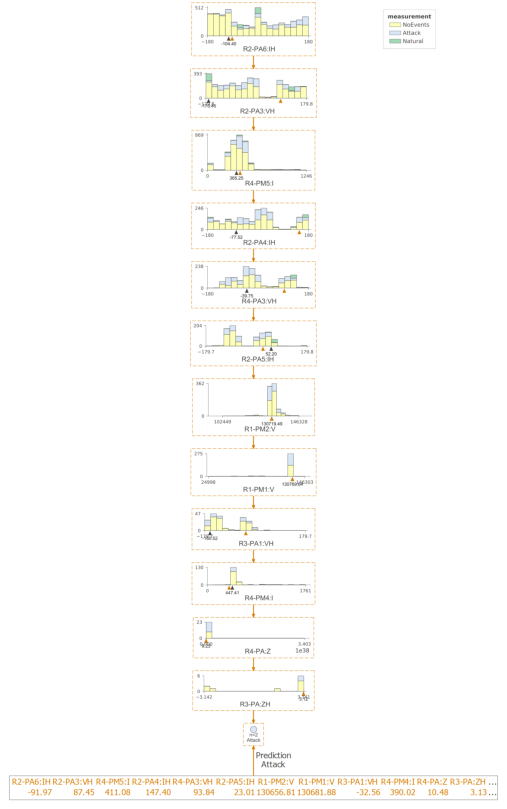
\includegraphics[width=.9\paperwidth, height=.9\textheight]{images/dtreeviz}}
%     \caption{dtreeviz's visualisation of the prediction path for Natural event mispredicted as Attack}
%     \label{fig:dtreeviz}
% \end{figure}



\subsection{Summary}
It can be concluded that ELI5 is the most versatile package compared to others, especially because it enables both global and local interpretations and does not limit its support to scikit-learn, plus it has LIME integrated in it. YellowBrick on other hand adds the possibility to analyse from a statistical view the features available in the dataset. Finally comes Treeinterpreter and dtreeviz that are interesting tools when analysing especially Decision Trees. A summary of the most import features of all 5 packages is shown in table \ref{tab:comp}.

\begin{table}[H]
    \centering
    \caption{Comparison of tools for model analysis} \label{tab:comp}
    \begin{tabular}{lccccc} \toprule
        & LIME & ELI5 & YellowBrick & Treeinterpreter & dtreeviz \\\midrule
        Global interpretation & \xmark & \cmark & \cmark & \xmark & \xmark \\
        Local interpretation & \cmark & \cmark & \xmark & \cmark & \cmark \\
        Black-box models support & \cmark & \cmark & \cmark & \xmark & \xmark \\
        Features' statistical analysis & \xmark & \xmark & \cmark & \xmark & \xmark \\
        Works only with scikit-learn & \cmark & \xmark & \cmark & \cmark & \cmark \\
        Decision Trees graphical visualisation & \xmark & \xmark & \xmark & \xmark & \cmark \\
        \bottomrule
    \end{tabular}
\end{table}

\section{Features' importance determination}
%Lime
For the rest of the chapter LIME was chosen to determine the features' importance because of it working with all black-box models available in scikit-learn. The capabilities of LIME were sufficient and that is why ELI5 was not used in his place.

Since in this case the explanations of single samples are not really interesting, an attempt to generalize the results was made: Lime explainer was run on 100 false predictions of a chosen class. The results are concatenated together, and for all the features that are duplicated, the importance is calculated as the mean value of the importances and only one entry is kept with the calculated average importance. This algorithm was also run omitting the differentiation between classes. The results, reduced to 10 entries each, are shown below.

For NoEvents class:
\begin{verbatim}
                                     importance
 feature                                      
 R2-PM1:V > 130872.03                -0.013013
 R3-PA2:VH <= -93.75                 -0.011134
 R2-PA7:VH <= -101.20                -0.010218
 R3-PM2:V > 130431.15                -0.009583
 R2-PM7:V > 130857.40                -0.009377
 ...                                       ...
 R3-PM5:I <= 330.70                   0.005762
 0.00 < R1-PA12:IH <= 32.04           0.007514
 128762.21 < R2-PM1:V <= 129859.49    0.007776
 R3-PM2:V <= 128425.29                0.007998
 R4-PA5:IH > 115.38                   0.008534
 
 [361 rows x 1 columns]
\end{verbatim}

For Attack class:
\begin{verbatim}
                                   importance
    feature                                 
    R3-PA2:VH > 113.97             -0.012837
    -97.10 < R4-PA7:VH <= -35.66   -0.010994
    -97.43 < R1-PA7:VH <= -35.85   -0.010306
    R2-PA2:VH > 114.00             -0.009730
    R3-PM2:V <= 128425.29          -0.006914
    ...                                  ...
    R3-PA2:VH <= -93.75             0.008307
    R3-PA7:VH <= -101.22            0.008676
    R2-PM1:V > 130872.03            0.009242
    R3:S > 0.00                     0.010717
    R2-PA7:VH <= -101.20            0.014018
    
    [380 rows x 1 columns]
\end{verbatim}

For Natural class: 
\begin{verbatim}
                            importance
    feature                          
    R2-PA5:IH <= -74.26     -0.003613
    R4-PM3:V > 132484.78    -0.002835
    R4-PM2:V > 132187.18    -0.002437
    R2-PM7:V <= 128751.24   -0.002290
    R2-PM1:V <= 128762.21   -0.002151
    ...                           ...
    R1-PA1:VH > 71.28        0.003518
    R2-PM7:V > 130857.40     0.003693
    R2-PA5:IH > 63.30        0.004103
    R3:F > 60.00             0.004873
    R2:F > 60.00             0.005168
    
    [331 rows x 1 columns]]
\end{verbatim}

For all classes:
\begin{verbatim}
                                 importance
    feature                                
    R3-PM2:V <= 128425.29         -0.006715
    R2-PA7:VH > 65.91             -0.006353
    R3-PM5:I <= 330.70            -0.006009
    -40.44 < R3-PA1:VH <= 65.76   -0.005808
    R3-PA4:IH <= -65.22           -0.005764
    ...                                 ...
    R2-PA3:VH <= -75.28            0.005588
    R3-PA4:IH > 102.49             0.005723
    R4-PA1:VH > 71.50              0.007481
    R3-PM2:V > 130431.15           0.008501
    R2-PM1:V > 130872.03           0.009070
    
    [331 rows x 1 columns]
\end{verbatim}